\subsection{Модификация базы данных REACLIB} \label{sec:ratelib}
\subsubsection{Представление скоростей реакций в REACLIB}
В настоящей работе скорости нейтронных захватов, полученные при помощи программы TALYS с использованием различных таблиц теоретических масс нейтроноизбыточных ядер, подставлялись в библиотеку астрофизических реакций REACLIB~\cite{reaclib2010}. В REACLIB скорость реакции $\lambda$ задается семью параметрами $a_i$ функции температуры $T$ (в ГК):
\begin{equation}
    \lambda = \exp \left[ a_0 + \sum_{i=1}^5 a_i T^{\frac{2i-5}{3}} + a_6 \ln T \right]
    \label{eq:reaclib_format}
\end{equation}

Программа TALYS выдает результаты расчета скоростей в виде таблицы в астрофизическом диапазоне температур от $10^5$ до $10^{10}$~К. Для представления полученных нами скоростей реакций в формате REACLIB их необходимо аппроксимировать с помощью функции~(\ref{eq:reaclib_format}). В настоящей работе для этого использовался нелинейный метод наименьших квадратов с минимизацией по методу Левенберга--Марквардта (см., например,~\cite{levenberg1944}), реализованный в пакете научных вычислений scipy~\cite{scipy2020}. 

Аппроксимация проводилась по равномерной сетке температур от $0.5$ до $6$~ГК с шагом $0.2$~ГК. Мы взяли не весь диапазон температур, в котором TALYS выдает результаты, чтобы добиться наилучшей точности в интересующей нас области $1-5$~ГК. Выбор длины шага обусловлен тем, что функция~(\ref{eq:reaclib_format}) оказалась склонна к осцилляциям на концах диапазона аппроксимации, возникающим при слишком густой сетке, а при указанном шаге они почти исчезают. Скорости реакции $(n,\gamma)$ на нейтроноизбыточных изотопах индия, тербия и свинца, полученные нами с помощью программы TALYS и аппроксимированные для представления в формате REACLIB, показаны на рис.~\ref{fig:ng_approx}. 

\begin{figure}
  \centering
  \begin{subfigure}{0.48\textwidth}
    \centering
    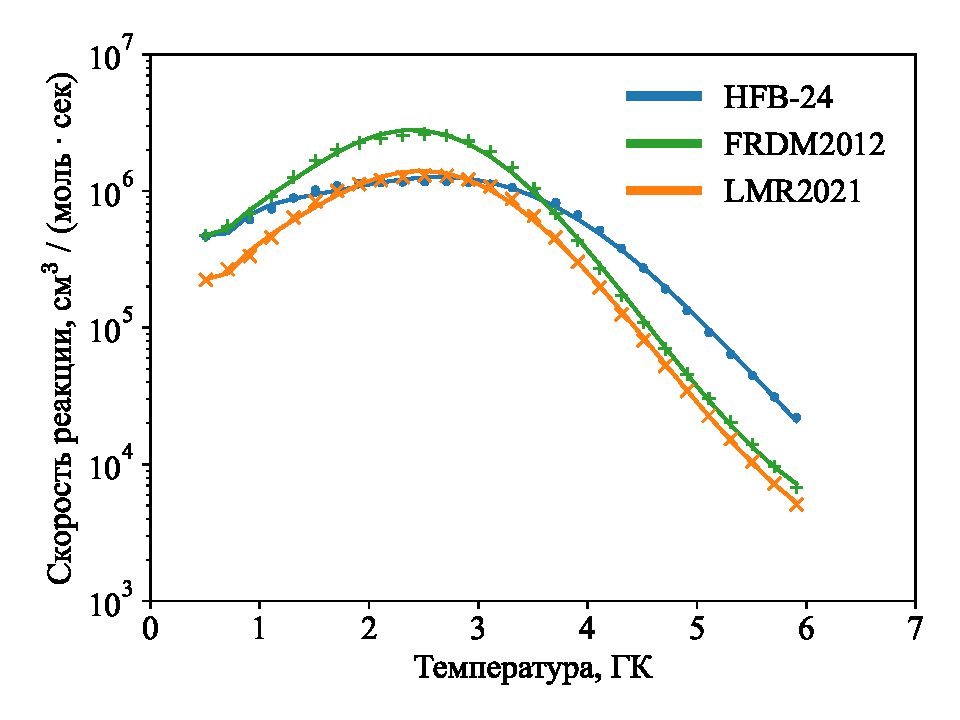
\includegraphics[width=\textwidth]{pics/ng_fit_pb236.pdf}
    \caption{${}^{236}$Pb}
  \end{subfigure}
  \hfil
  \begin{subfigure}{0.48\textwidth}
    \centering
    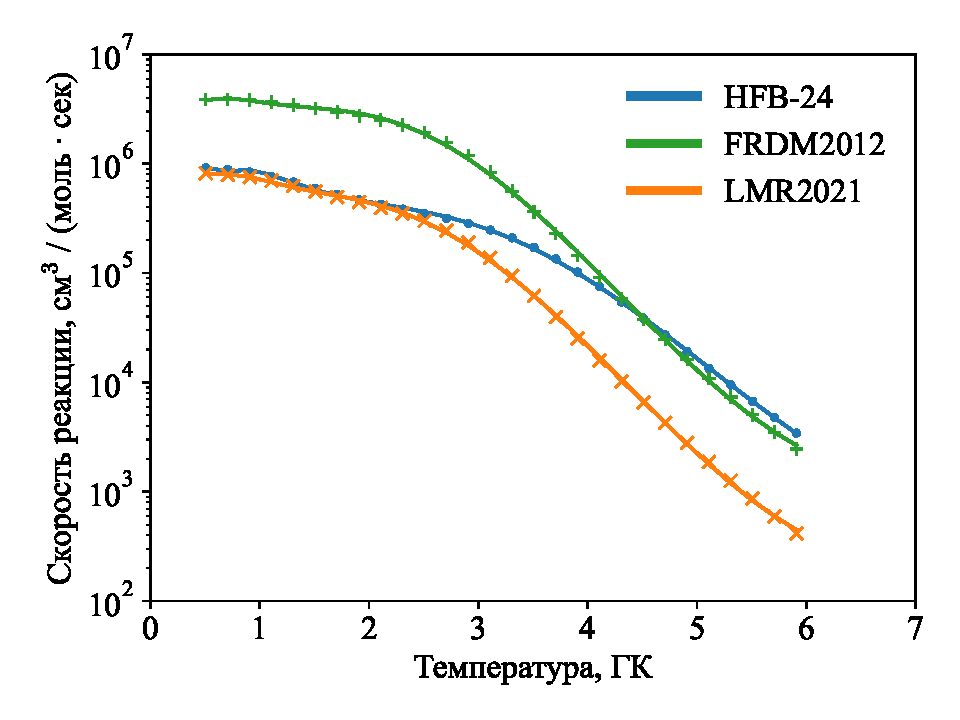
\includegraphics[width=\textwidth]{pics/ng_fit_pb237.pdf}
    \caption{${}^{237}$Pb}
  \end{subfigure}
  \caption{Скорости реакции $(n,\gamma)$ на нейтроноизбыточных изотопах свинца ${}^{236}$Pb и ${}^{237}$Pb, полученные с помощью программы TALYS с использованием различных массовых моделей, и результаты их аппроксимации функцией~(\ref{eq:reaclib_format}).}
  \label{fig:ng_approx}
\end{figure}

\subsubsection{Пакет ratelib}
Для упрощения работы с базами данных астрофизических скоростей реакций в формате REACLIB в рамках настоящей работы на языке Python был реализован и опубликован в открытом доустпе пакет ratelib, доступный для загрузки с помощью каталога Python-пакетов PyPI\footnote{\href{https://pypi.org/project/ratelib/}{https://pypi.org/project/ratelib/}}. Пакет ratelib поддерживает загрузку базы данных из текстового файла, представление нуклидов, скоростей реакций и их коллекций в виде объектов языка Python, аппроксимацию таблиц скоростей реакций с помощью функции~(\ref{eq:reaclib_format}) и вывод данных в формате REACLIB в текстовый файл. В настоящей работе все модификации библиотеки REACLIB, в том числе аппроксимации функции~\ref{eq:reaclib_format}, выполнены при помощи пакета ratelib.

\subsubsection{Критерий нейтроноизбыточности}
Подставляя скорости $(n,\gamma)$ в библиотеку REACLIB, мы ограничивались только реакциями на нейтроноизбыточных изотопах. Для других ядер стандартные значения скоростей оставлялись неизменными.

То, является ли изотоп нейтроноизбыточным, определялось ненулевым значением скорости распада, а также отношением числа нейтронов к протонам. Продифференцировав формулу Вайцзеккера по числу нейтронов $N$, можно найти простое условие максимума энергии связи:
\begin{equation}
  \displaystyle
  \frac{N}{Z} = c_1 + c_2 A^{2/3}
  \label{eq:nzratio}
\end{equation}
Хотя параметры $c_1$ и $c_2$ можно получить из известных значений коэффициентов формулы Вайцзеккера, для надежности мы аппроксимировали их, используя список стабильных ядер, полученный из базы данных NUBASE2020~\cite{kondev2021}.
